\documentclass{article}

% Packages
\usepackage[margin=0.8in]{geometry}
\usepackage[utf8]{inputenc}
\usepackage{dsfont}
\usepackage{pgfplots}
\usepackage{algorithm}
\usepackage{algorithmic}
\usepackage{amsmath}
\usepackage{amssymb}
\usepackage{subfig}
\usepackage{amsfonts}
\usepackage{tikz}
\usepackage{titling}
\renewcommand\maketitlehooka{\null\mbox{}\vfill}
\renewcommand\maketitlehookd{\vfill\null}

% Custom settings
\setlength{\parskip}{0.75em}  % Paragraph spacing
\setcounter{section}{-1} % Page numbers to start on page 1
\setlength\parindent{0pt} % Remove indenting from entire file
\def\layersep{2.5cm}

\title{CS229 Machine Learning}
\author{Stanford University/Coursera}
\date{Andrew Ng}

% For page counter to start on p.2
% \pagenumbering{gobble}

% Plot package backwards compatibility
\pgfplotsset{compat=1.14}

\begin{document}

    % Title page
    \begin{titlingpage}
        \maketitle
        \centering
        \vfill
        {\large{Matteo Esposito}}
    \end{titlingpage}

    \newpage

    \section{Introduction}

        \textit{This document is a compilation of notes from the machine learning coursera MOOC taught by Prof. Andrew Ng of Stanford University
        offered by Coursera.}
        \par
        % Intro notes
        \textbf{Supervised learning} problems are categorized into "regression" and "classification" problems. In a regression problem, 
        we are trying to predict results within a continuous output, meaning that we are trying to map input variables to some 
        continuous function. In a classification problem, we are instead trying to predict results in a discrete output. In other words, 
        we are trying to map input variables into discrete categories.
        \par
        \textbf{Unsupervised learning} allows us to approach problems with little or no idea what our results should look like. 
        We can derive structure from data where we don't necessarily know the effect of the variables.
        We can derive this structure by clustering the data based on relationships among the variables in the data.
        With unsupervised learning there is no feedback based on the prediction results.
        \par
        From this point, we will use $X$ to denote the space of input values, and $Y$ to denote the space of output values. In this example, $X = Y = \mathbb{R}$.
        \par
        To describe the supervised learning problem slightly more formally, our goal is, given a training set, 
        to learn a function $h : X \longrightarrow Y$ so that $h(x)$ is a “good” predictor for the corresponding value of y. For historical reasons, this 
        function $h$ is called a hypothesis. 
        
        \subsection{Cost Function}
            
            We can measure the accuracy of our hypothesis function by using a \textbf{cost function}. This takes an average difference (actually a fancier version of an average)
            of all the results of the hypothesis with inputs from x's and the actual output y's.
            % Cost function
            \begin{align*}
               J(\theta_{0},\theta_{1}) = \frac{1}{2m}\sum_{i=1}^{m}(\hat{y_i} - y_i)^2 = \frac{1}{2m}\sum_{i=1}^{m}(h_{\theta}(x_i)- y_i)^2
            \end{align*}
            This function is otherwise called the "Squared error function", or "Mean squared error". The mean is halved $\left(\frac{1}{2}\right)$
            as a convenience for the computation of the gradient descent, as the derivative term of the square function will cancel out the $\left(\frac{1}{2}\right)$ 
            term. $J$ will be 0 if we can achieve a perfect fit (not always possible, and when possible, will probably mean overfitting). We can use a contour plot to visualize the minimizing of the cost function.
            % Contour plot
            \vspace{12pt}
            \begin{center}
                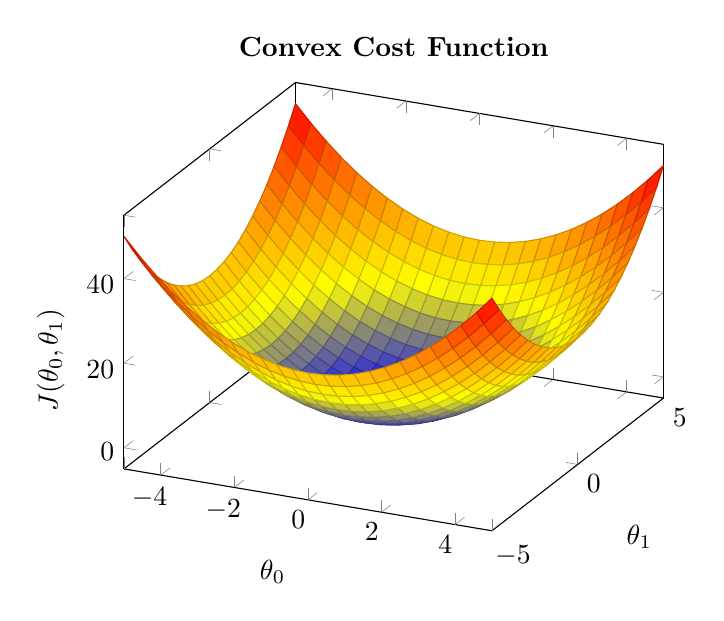
\begin{tikzpicture}
                    \begin{axis}[
                        title={\textbf{Convex Cost Function}},
                        xlabel = {$\theta_{0}$},
                        ylabel = {$\theta_{1}$},
                        zlabel = {$J(\theta_{0},\theta_{1})$}]
                        \addplot3[surf,] {x^2 + y^2};
                    \end{axis}
                \end{tikzpicture}
            \end{center}
            
        \subsection{Gradient Descent}

            \begin{algorithm}
                \caption{General Gradient Descent}
                \begin{algorithmic}
                    \FOR{$n >= 1$}
                        \STATE $n = $number of features, $m = $number of samples
                        \STATE \emph{repeat until convergence}:
                        \STATE \hspace{12pt}$\theta_j \gets \theta_j - \alpha\frac{\partial}{\partial\theta_j}J(\theta_{0},\theta_{1}) =
                                            \theta_j - \alpha\frac{1}{m}\sum_{i=1}^{m}((h_{\theta}(x^{(i)})-y^{(i)})x_j^{(i)})$
                    \ENDFOR
                \end{algorithmic}
            \end{algorithm}
            
            We will know that we have succeeded when our cost function is at the very bottom of the pits in our graph, i.e. when its value is the minimum. 
            
            The way we do this is by taking the derivative (the tangential line to a function) of our cost function. 
            The slope of the tangent is the derivative at that point and it will give us a direction to move towards.
            We make steps down the cost function in the direction with the steepest descent. 
            The size of each step is determined by the parameter $\alpha$, which is called the learning rate.
            
    % Week 1-2
    \section{Linear Regression}
        
        The standard form of the hypothesis function for linear regression is the following:
        \begin{align*}
            h_{\theta}(x) = \theta_0 + \theta_1x
        \end{align*}
        In the case of linear regression we use MSE as the cost function $J(\theta)$.
        \begin{align*}
            \frac{\partial}{\partial\theta_j}J(\theta) &= \frac{\partial}{\partial\theta_j}\frac{1}{2}(h_{\theta}(x)-y)^2 \\
            &= 2\cdot\frac{1}{2}(h_{\theta}(x)-y)\cdot\frac{\partial}{\partial\theta_j}(h_{\theta}(x)-y) \\
            &= (h_{\theta}(x)-y)\cdot\frac{\partial}{\partial\theta_j}\left(\sum_{i=0}^{n}\theta_ix_i-y\right) \\
            &= (h_{\theta}(x)-y)x_j
        \end{align*}
        
        \begin{algorithm}
            \caption{Gradient Descent for Linear Regression}
            \begin{algorithmic}
                \STATE $n = $number of features, $m = $number of samples
                \STATE \emph{repeat until convergence}:
                \STATE \hspace{12pt}$\theta_0 \gets \theta_0 - \alpha\frac{1}{m}\sum_{i=1}^{m}(h_{\theta}(x^{(i)})-y^{(i)})$
                \STATE \hspace{12pt}$\theta_1 \gets \theta_1 - \alpha\frac{1}{m}\sum_{i=1}^{m}((h_{\theta}(x^{(i)})-y^{(i)})x_1^{(i)})$
            \end{algorithmic}
        \end{algorithm}
        
        The point of all this is that if we start with a guess for our hypothesis and then repeatedly apply these gradient descent equations, 
        our hypothesis will become more and more accurate.
        \par
        \underline{Note:} In the general case, we know that there is a possibility for gradient descent to fall into a local minimum trap, this is however impossible in the
        case of linear regression. There is a single global minimum and no local minima.

        \newpage 

        \subsection{Multivariate Linear Regression}

        The multivariable form of the hypothesis function accommodating these multiple features is as follows:
        \begin{align*}
            h_{\theta}(x) = \theta_0 + \theta_1x_1 +  \theta_1x_2 + \ldots + \theta_nx_n
        \end{align*}

        % Weird indent
        This can be represented as follows:
        \begin{align*}
            \begin{bmatrix}
                \theta_0   & \theta_1 & \theta_2 & \dots & \theta_n
            \end{bmatrix}
            \begin{bmatrix}
                x_{0} \\
                x_{1} \\
                \vdots \\
                x_{n} 
            \end{bmatrix}  =  \theta^Tx
        \end{align*}

        Here we use the general gradient descent algorithm.

        \subsection{Feature Scaling}

        We can speed up gradient descent by having each of our input values in roughly the same range. This is because 
        $\theta$ will descend quickly on small ranges and slowly on large ranges, and so will oscillate inefficiently
        down to the optimum when the variables are very uneven. Scaling features becomes increasingly important when 
        creating features (i.e. in the case of polynomial regression).
        \par
        Two techniques to help with this are \textbf{feature scaling} and \textbf{mean normalization}. 
        \begin{itemize}
            \item Feature scaling involves dividing the input values by the range (i.e. the maximum value minus the minimum value) of the input variable, 
                  resulting in a new range of just 1. 
            \item Mean normalization involves subtracting the average value for an input variable from the values for 
                  that input variable resulting in a new average value for the input variable 
                  of just zero. To implement both of these techniques, adjust your input values as shown in this formula, where $s_i$ is the range our
                  standard deviation.
            \begin{align*}
                x_i \longleftarrow \frac{x_i-\mu_i}{s_i}
            \end{align*}
        \end{itemize}

        \subsection{Learning Rate}

            To monitor/make sure gradient descent is working correctly, we can plot the value of $\min_{\theta}J(\theta)$ vs. 
            the number of iterations and hope to see a reasonably paced decrease in the minimum value achieved.
            \begin{center}
                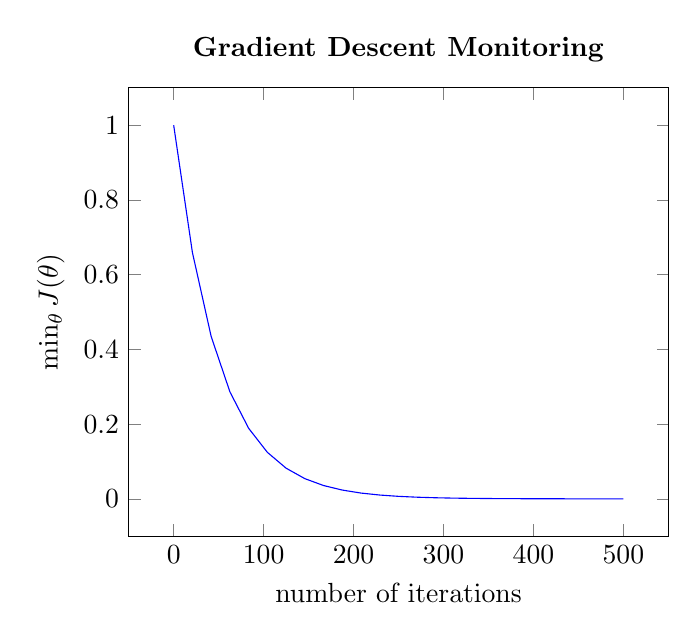
\begin{tikzpicture}
                    \begin{axis}[
                        title={\textbf{Gradient Descent Monitoring}},
                        xlabel = {number of iterations},
                        ylabel = {$\min_{\theta}J(\theta)$}]
                        \addplot[draw=blue, sharp plot][domain=0:500] {e^-x/50};
                    \end{axis}
                \end{tikzpicture}
            \end{center}
        
            Properties of the learning rate $\alpha$:
            \begin{itemize}
                \item It has been proven that if learning rate $\alpha$ is sufficiently small, then $J(\theta)$ will decrease on every iteration.
                \item If $\alpha$ is too small: slow convergence.
                \item If $\alpha$ is too large: may not decrease on every iteration and thus may not converge.
            \end{itemize}

        \subsection{Normal Equation}

            Gradient descent gives one way of minimizing $J$. Let’s discuss a second way of doing so, this time performing the minimization explicitly and
            without resorting to an iterative algorithm. In the "Normal Equation" method, we will minimize $J$ by explicitly taking its derivatives with 
            respect to the $\theta_j$’s, and setting them to zero. This allows us to find the optimum theta without iteration. The normal equation formula is given below:
            \begin{align*}
                \theta = (X^TX)^{-1}X^Ty
            \end{align*}
            There is no need to do feature scaling with the normal equation. With the normal equation, computing the inversion has complexity 
            $\mathcal{O}(n^3)$, whereas gradient descent has time complexity $\mathcal{O}(kn^2)$ . So if we have a very large number of features, the normal equation will be slow. In practice, when n exceeds 
            10,000 it might be a good time to go from a normal solution to an iterative process.
            \par
            \underline{Note:} Non-invertibility/singularity of the feature/design matrix $X$ can become an issue when using the 
            normal equation, but only in cases where the number of samples is less than or equal to the number of features $(m < n)$. 
    
    % Week 3
    \section{Logistic Regression}

        \subsection{Classification and Representation}
            Binary classifiers are widely used in machine learning applications, to predict output, or probability of output where the 
            range of possible values is a small set of discrete values (e.g. 0 \& 1). We technically can use linear regression
            to map all predictions greater than 0.5 to 1 and 0 otherwise. For binary classification purposes, intuitively, it doesn’t make sense for $h_\theta(x)$
            to take values larger than 1 or smaller than 0 when we know that $y \in \{0, 1\}$.  To fix this, let’s change the form 
            for our hypotheses $h_\theta(x)$ to satisfy $0 \leq h_\theta (x) \leq 1$. This is accomplished by plugging $\theta^Tx$ into the \textbf{Logistic Function}.
            Our new form uses the "Sigmoid Function," also called the "Logistic Function":

            \vspace{-6pt}

            \begin{align*}
                h_{\theta}(x) = g(\theta^Tx) \hspace{3em} z = \theta^Tx \hspace{3em} g(z) = \frac{1}{1-e^{-z}} \\
            \end{align*}

            \begin{center}
                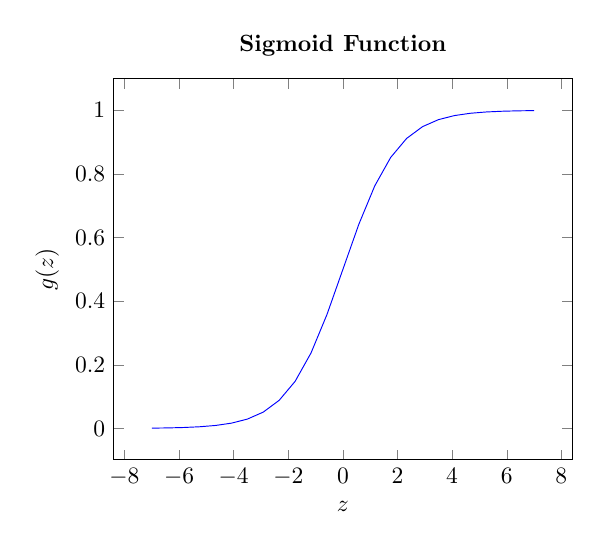
\begin{tikzpicture}[scale=0.85]
                    \begin{axis}[
                        title={\textbf{Sigmoid Function}},
                        xlabel = {$z$},
                        ylabel = {$g(z)$}]
                        \addplot[draw=blue, sharp plot][domain=-7:7] {1/(1+e^-x)};
                    \end{axis}
                \end{tikzpicture}
            \end{center}

            The function $g(z)$, shown here, maps any real number to the $(0, 1)$ interval, making it useful for transforming an 
            arbitrary-valued function into a function better suited for classification.

            $h_\theta(x)$ will give us the probability that our output is 1. For example, $h_\theta(x) = 0.7$
            gives us a probability of 70\% that our output is 1. Our probability that our prediction is 0 is just the complement of 
            our probability that it is 1 (e.g. if probability that it is 1 is 70\%, then the probability that it is 0 is 30\%).

            \begin{center}
                $\begin{cases}
                    h_\theta(x) = P(y=1|x;0) = 1 - P(y=0|x;0) \\
                    P(y=1|x;0) + P(y=0|x;0) = 1  
                \end{cases}$
            \end{center}

            The decision boundary is the line that separates the area where y = 0 and where y = 1. 
            It is created by our hypothesis function. Example:

            \begin{align*}
                \theta = 
                \begin{bmatrix}
                    5 \\
                    -1 \\
                    0
                \end{bmatrix} \Longrightarrow y=1 \text{ if } 5 + (-1)x_1 + 0x_2 \geq 0 \therefore x1 \leq 5
            \end{align*}

            In this case, our decision boundary is a straight vertical line placed on the graph where $x_1 = 5$, and everything
            to the left of that denotes $y = 1$, otherwise 0.

            Again, the input to the sigmoid function $g(z) (e.g. \theta^TX)$ doesn't need to be linear, and could be a function that
            describes a circle $z = \theta + \theta x_1^2 + \theta_2x_2^2$ or any shape to fit our data.

        \subsection{Logistic Regression Model}

            We cannot use the same cost function that we use for linear regression because the Logistic Function will cause the output to be wavy, 
            causing many local optima. In other words, it will not be a convex function. Instead, our cost function for logistic regression looks like:
        
            \begin{align*}
                J(\theta) = \frac{1}{m} Cost(h_{\theta}(x^{(i)}),y^{(i)}) 
            \end{align*}
            \vspace{-6pt}
            \begin{align*}
                \begin{cases}
                    Cost(h_{\theta}(x),y) = -log(h_{\theta}(x)) & \mbox{if } y = 1 \\
                    Cost(h_{\theta}(x),y) = -log(1-h_{\theta}(x)) & \mbox{if } y = 0 \\
                \end{cases}    
            \end{align*}
            
            \begin{center}
                \centering
                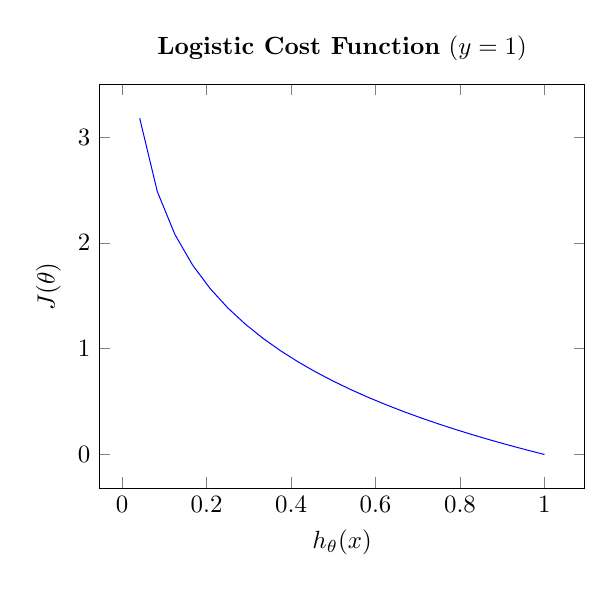
\begin{tikzpicture}[scale=0.9]
                    \begin{axis}[
                        title={\textbf{Logistic Cost Function} $(y=1)$},
                        xlabel = {$h_{\theta}(x)$},
                        ylabel = {$J(\theta)$}]
                        \addplot[draw=blue, sharp plot][domain=0:1] {-ln(x)};
                    \end{axis}
                \end{tikzpicture}
                \qquad
                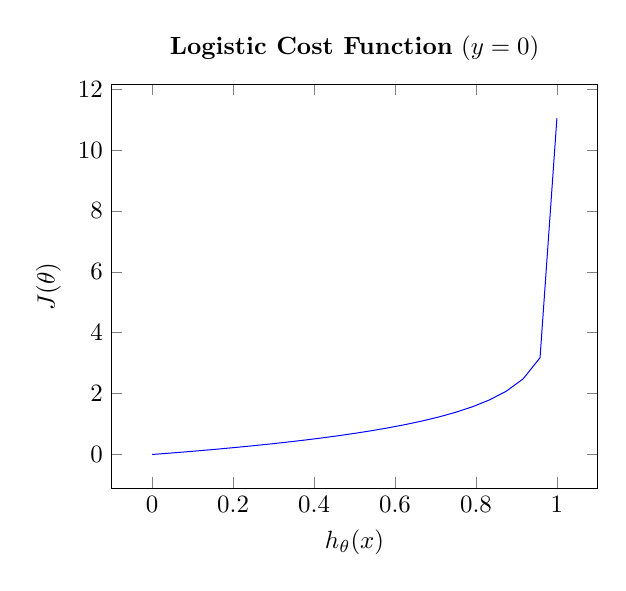
\begin{tikzpicture}[scale=0.9]
                    \begin{axis}[
                        title={\textbf{Logistic Cost Function} $(y=0)$},
                        xlabel = {$h_{\theta}(x)$},
                        ylabel = {$J(\theta)$}]
                        \addplot[draw=blue, sharp plot][domain=0:1] {-ln(1-x)};
                    \end{axis}
                \end{tikzpicture}
            \end{center}

            If our correct answer 'y' is 0, then the cost function will be 0 if our hypothesis function also outputs 0. 
            If our hypothesis approaches 1, then the cost function will approach infinity.

            If our correct answer 'y' is 1, then the cost function will be 0 if our hypothesis function outputs 1. 
            If our hypothesis approaches 0, then the cost function will approach infinity.
            \begin{align*}
                \begin{cases}
                    Cost(h_{\theta}(x),y) = 0 \text{ if } h_{\theta}(x) = y \\
                    Cost(h_{\theta}(x),y) \longrightarrow \infty \text{ if } y = 0 \text{ and } h_{\theta}(x) \longrightarrow 1 \\
                    Cost(h_{\theta}(x),y) \longrightarrow \infty \text{ if } y = 1 \text{ and } h_{\theta}(x) \longrightarrow 0
                \end{cases}
            \end{align*}
            We can compress our cost function's two conditional cases into one case:
            \begin{align*}
                Cost(h_{\theta}(x),y) = -ylog(h_{\theta}(x)) - (1-y)log(1-h_{\theta}(x))
            \end{align*}
            Therefore,
            \begin{align*}
                J(\theta) = -\frac{1}{m}\sum_{i=1}^{m}[y^{(i)}log(h_{\theta}(x^{(i)})) + (1-y^{(i)})log(1-h_{\theta}(x^{(i)})]
            \end{align*}

        \subsection{Multiclass Classification}

            Now we will approach the classification of data when we have more than two categories. Instead of $y = \{0,1\}$ we will expand our definition so that $y = \{0,1...n\}$.

            Since $y = \{0,1...n\}$, we divide our problem into $n+1$ (+1 because the index starts at 0) binary classification problems; in each one, we predict 
            the probability that 'y' is a member of one of our classes.

            \begin{align*}
                \begin{cases}
                    y \in \{0,1,\ldots, n\} \\
                    h_{\theta}^{(0)}(x) = P(y=0|x;\theta) \\
                    h_{\theta}^{(1)}(x) = P(y=1|x;\theta) \\
                    \ldots \\
                    h_{\theta}^{(n)}(x) = P(y=n|x;\theta) \\
                \end{cases}
                \Longrightarrow \; \; \; prediction = \max_{i}(h_{\theta}^{(i)}(x))
            \end{align*}

            We are basically choosing one class and then lumping all the others into a single second class. We do this repeatedly, applying binary logistic 
            regression to each case, and then use the hypothesis that returned the highest value as our prediction.
        
        \subsection{Solving the Problem of Overfitting}

            \textbf{Underfitting}, or high bias, is when the form of our hypothesis function h maps poorly to the trend of the data. 
            It is usually caused by a function that is too simple or uses too few features. At the other extreme, \textbf{overfitting}, or high variance, 
            is caused by a hypothesis function that fits the available data but does not generalize well to predict new data. It is usually caused by 
            a complicated function that creates a lot of unnecessary curves and angles unrelated to the data.

            This terminology is applied to both linear and logistic regression. There are two main options to address the issue of overfitting:
        
            \begin{enumerate}
                \item Reduce the number of features
                    \begin{itemize}
                        \item Manually select which features to keep
                        \item Use a model selection algorithm        
                    \end{itemize}
                \item Regularization
                    \begin{itemize}
                        \item Keep all the features, but reduce the magnitude of parameters $\theta_j$.
                        \item Regularization works well when we have a lot of slightly useful features.      
                    \end{itemize}
            \end{enumerate}

            If we have overfitting from our hypothesis function, we can reduce the weight that some of the terms in our function carry by increasing their cost.
            So, lets say we wanted to make the following function more quadratic:
            \begin{align*}
                 h_{\theta}(x)= \theta_{0} + \theta_{1}x + \theta_{2}x^2 + \theta_{3}x^3 + \theta_{4}x^4
            \end{align*}
            We want to eliminate the influence of $\theta_3x^3$ and $\theta_4x^4$. Without actually getting rid of these features or chaning the form
            of our hypothesis, we can instead modify our cost function:
            \begin{align*}
                \min_{\theta}\frac{1}{2m}\sum_{i=1}^m(h_{\theta}(x^{(i)})-y^{(i)})^2 + 1000\cdot\theta_3^2 + 1000\cdot\theta_4^2
            \end{align*}
            We've artificially inflated the cost of $\theta_3$ and $\theta_4$.
            Now, in order for the cost function to get close to zero, we will have to reduce the values of
            $\theta_3$ and $\theta_4$ to near zero. This will make our cost function more quadratic.

            We could also regularize all of our theta parameters in a single summation as:
            \begin{align*}
                \min_{\theta}\frac{1}{2m}\sum_{i=1}^m(h_{\theta}(x^{(i)})-y^{(i)})^2 + \lambda\sum_{j=1}^{n}\theta_j^2        
            \end{align*}
            The $\lambda$, or lambda, is the regularization parameter. It determines how much the costs of our theta parameters are inflated.

            Using the above cost function with the extra summation, we can smooth the output of our hypothesis function to reduce overfitting. If lambda is chosen 
            to be too large, it may smooth out the function too much and cause underfitting.

            \begin{algorithm}
                \caption{Regularized Gradient Descent}
                \begin{algorithmic}
                    \STATE $n = $number of features, $m = $number of samples
                    \STATE \emph{repeat until convergence}:
                    \STATE \hspace{12pt}$\theta_0 \gets \theta_0 - \alpha\frac{1}{m}\sum_{i=1}^{m}(h_{\theta}(x^{(i)})-y^{(i)})x_0^{(i)}$
                    \STATE \hspace{12pt}$\theta_j \gets \theta_j - \alpha\left[\left(\frac{1}{m}\sum_{i=1}^{m}((h_{\theta}(x^{(i)})-y^{(i)})x_j^{(i)}\right) + \frac{\lambda}{m}\theta_j\right]$ \qquad $j \in \{1,2,\ldots,n\}$
                \end{algorithmic}
            \end{algorithm}    

    % Week 4
    \section{Neural Networks}

        At a very simple level, neurons are basically computational units that take inputs 
        (dendrites) as electrical inputs (called "spikes") that are channeled to outputs (axons). In our model, 
        our dendrites are like the input features $x_1 \ldots x_n$, nd the output is the result of our hypothesis function. In this model our $x_0$
        input node is sometimes called the "bias unit." It is always equal to 1. In neural networks, 
        we use the same logistic function as in classification, $\frac{1}{1+e^{-\theta^Tx}}$, yet we sometimes call it a sigmoid (logistic)
        \textbf{activation} function. In this situation, our theta parameters are sometimes called "weights".

        Our input nodes (layer 1), also known as the "input layer", go into another node (layer 2), which finally outputs the hypothesis function, known as the "output layer".

        We can have intermediate layers of nodes between the input and output layers called the "hidden layers."

        \newpage
        In this example, we label these intermediate or "hidden" layer nodes $a_0^2 \ldots a_n^2$ and call them "activation units".

        If we had one hidden layer, it would look like:

        \begin{align*}
            \begin{bmatrix}
                x_0 \\
                x_1 \\
                x_2 \\
                x_3
            \end{bmatrix} \longrightarrow
            \begin{bmatrix}
                a_1^{(2)} \\
                a_2^{(2)} \\
                a_3^{(2)} 
            \end{bmatrix} \longrightarrow h_{\theta}(x)
        \end{align*}
        
        The values for each of the "activation" nodes is obtained as follows:

        \begin{align*}
            \begin{cases}
                a_1^{(2)} = g(\theta_{10}^{(1)}x_0 + \theta_{11}^{(1)}x_1 + \theta_{12}^{(1)}x_2 + \theta_{13}^{(1)}x_3) \\
                a_2^{(2)} = g(\theta_{20}^{(1)}x_0 + \theta_{21}^{(1)}x_1 + \theta_{22}^{(1)}x_2 + \theta_{23}^{(1)}x_3) \\
                a_3^{(2)} = g(\theta_{30}^{(1)}x_0 + \theta_{31}^{(1)}x_1 + \theta_{32}^{(1)}x_2 + \theta_{33}^{(1)}x_3)
            \end{cases} \longrightarrow \; \;h_{\theta}(x) = a_1^{(3)} = g(\theta_{10}^{(2)}a_0^{(2)} + \theta_{11}^{(2)}a_1^{(2)}+ \theta_{12}^{(2)}a_2^{(2)} + \theta_{13}^{(2)}a_3^{(2)})
        \end{align*}

        Our hypothesis output is the logistic function applied to the sum of the values of our activation nodes, 
        which have been multiplied by yet another parameter matrix $\theta^{(2)}$ containing the weights for our second layer of nodes.
        (Every layer gets its own matrix of weights, $\theta^{(j)}$).

        \begin{center}
            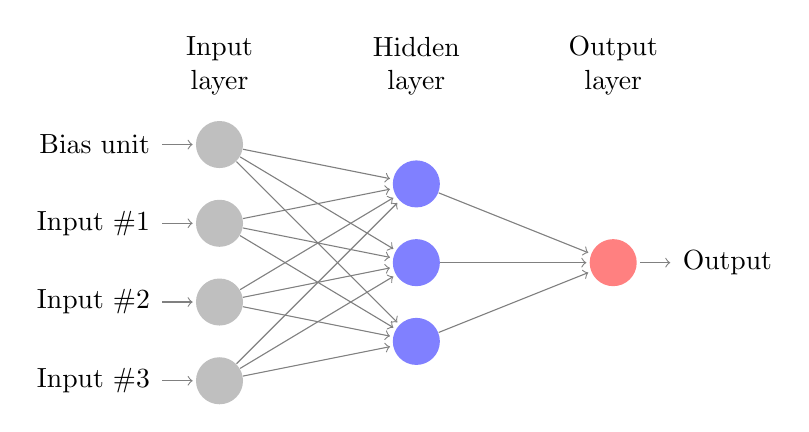
\begin{tikzpicture}[shorten >=1pt,->,draw=black!50, node distance=\layersep]
                \tikzstyle{every pin edge}=[<-,shorten <=1pt]
                \tikzstyle{neuron}=[circle,fill=black!25,minimum size=17pt,inner sep=0pt]
                \tikzstyle{input neuron}=[neuron, fill=gray!50];
                \tikzstyle{output neuron}=[neuron, fill=red!50];
                \tikzstyle{hidden neuron}=[neuron, fill=blue!50];
                \tikzstyle{annot} = [text width=4em, text centered]
            
                % Draw the bias unit node
                \foreach \name / \y in {0}
                % This is the same as writing \foreach \name / \y in {1/1,2/2,3/3,4/4}
                    \node[input neuron, pin=left:Bias unit] (I-\name) at (0,-\y-1.5) {};

                % Draw the input layer nodes
                \foreach \name / \y in {1,...,3}
                % This is the same as writing \foreach \name / \y in {1/1,2/2,3/3,4/4}
                    \node[input neuron, pin=left:Input \#\y] (I-\name) at (0,-\y-1.5) {};
            
                % Draw the hidden layer nodes
                \foreach \name / \y in {1,...,3}
                    \path[yshift=-1cm]
                        node[hidden neuron] (H-\name) at (\layersep,-\y cm) {};
            
                % Draw the output layer node
                \node[output neuron,pin={[pin edge={->}]right:Output}, right of=H-2] (O) {};
            
                % Connect every node in the input layer with every node in the
                % hidden layer.
                \foreach \source in {0,...,3}
                    \foreach \dest in {1,...,3}
                        \path (I-\source) edge (H-\dest);
            
                % Connect every node in the hidden layer with the output layer
                \foreach \source in {1,...,3}
                    \path (H-\source) edge (O);
            
                % Annotate the layers
                \node[annot,above of=H-1, node distance=1.5cm] (hl) {Hidden layer};
                \node[annot,left of=hl] {Input layer};
                \node[annot,right of=hl] {Output layer};
            \end{tikzpicture}
        \end{center}

        Here we can define a new variable $z_k^{(j)}$ that encompasses the parameters indide out $g$ function. In our
        previous example if we replaced by the variable $z$ for all the parameters we would get:

        \begin{align*}
            \begin{cases}
                a_1^{(2)} = g(z_1^{(2)}) \\
                a_2^{(2)} = g(z_3^{(2)}) \\
                a_3^{(2)} = g(z_3^{(2)})
            \end{cases}
        \end{align*}

        In other words, for layer $j=2$ and node $k$, the variable $z$ would be:
        \begin{align*}
            z_k^{(2)} = \theta_{k,0}^{(1)}x_0 + \theta_{k,1}^{(1)}x_1 + \ldots + \theta_{k,n}^{(1)}x_n
        \end{align*}
        We then get our final result with:
        \begin{align*}
            h_{\theta}(x) = a^{(j+1)} = g(z^{(j+1)}) \quad \text{where} \quad z^{(j+1)} = \theta^{(j)}a^{(j)}
        \end{align*}

        \underline{Note:} Here, $\theta$ represents a matrix of weights. In the last step we are performing a logistic regression.

        \subsection{Examples}

            We will showcase a simple example of applying neural networks by predicting $x_1$ AND $x_2$, which is the logical
            'and' operator and is only true if both $x_1$ and $x_2$ are 1 (or true).

            The graph of our function will look like:
            \begin{align*}
                \begin{bmatrix}
                    x_0 \\
                    x_1 \\
                    x_2
                \end{bmatrix} \longrightarrow \;
                \begin{bmatrix}
                    g(z^{(2)})
                \end{bmatrix} \longrightarrow \; h_{\theta}(x)
            \end{align*}
                
            Let's set our first theta matrix as:
            \begin{align*}
                \theta^{(1)} = [-30 \; \; \; 20 \; \; \; 20]
            \end{align*}
            This will cause the output of our hypothesis to only be positive if both $x_1$ and $x_2$ are 1. In other words:
            \begin{align*}
                h_{\theta}(x) = g(-30 + 20x_1 + 20x_2)
            \end{align*}
            \begin{align*}
                \begin{cases}
                    x_1 = 0 \text{  and  } x_2 = 0 \; \; \longrightarrow \; \; g(-30) \approx 0 \\
                    x_1 = 0 \text{  and  } x_2 = 1 \; \; \longrightarrow \; \; g(-10) \approx 0 \\
                    x_1 = 1 \text{  and  } x_2 = 0 \; \; \longrightarrow \; \; g(-10) \approx 0 \\
                    x_1 = 1 \text{  and  } x_2 = 1 \; \; \longrightarrow \; \; g(10) \approx 1 \text{  ***}
                \end{cases}
            \end{align*}
    % Week 5
    \newpage
    \section{Neural Networks/Backpropagation}



    % Week 6
    \section{Advice for Applying Machine Learning}



    % Week 7
    \section{Support Vector Machines}



    % Week 8
    \section{Unsupervised Learning}



    % Week 9
    \section{Anomaly Detection}



    % Week 10
    \section{Large Scale Machine Learning}



    % Week 11
    \section{Application Example: Photo OCR}




\end{document}
